\documentclass[11pt,a4paper]{report}
\usepackage[textwidth=37em,vmargin=30mm]{geometry}
\usepackage{calc,xunicode,amsmath,amssymb,paralist,enumitem,tabu,booktabs,datetime2,xeCJK,xeCJKfntef,listings}
\usepackage{tocloft,fancyhdr,tcolorbox,xcolor,graphicx,eso-pic,xltxtra,xelatexemoji}

\newcommand{\envyear}[0]{2025}
\newcommand{\envdatestr}[0]{2025-09-10}
\newcommand{\envfinaldir}[0]{webdb/2025/20250910/final}

\usepackage[hidelinks]{hyperref}
\hypersetup{
    colorlinks=false,
    pdfpagemode=FullScreen,
    pdftitle={Web Digest - \envdatestr}
}

\setlength{\cftbeforechapskip}{10pt}
\renewcommand{\cftchapfont}{\rmfamily\bfseries\large\raggedright}
\setlength{\cftbeforesecskip}{2pt}
\renewcommand{\cftsecfont}{\sffamily\small\raggedright}

\setdefaultleftmargin{2em}{2em}{1em}{1em}{1em}{1em}

\usepackage{xeCJK,xeCJKfntef}
\xeCJKsetup{PunctStyle=plain,RubberPunctSkip=false,CJKglue=\strut\hskip 0pt plus 0.1em minus 0.05em,CJKecglue=\strut\hskip 0.22em plus 0.2em}
\XeTeXlinebreaklocale "zh"
\XeTeXlinebreakskip = 0pt


\setmainfont{Brygada 1918}
\setromanfont{Brygada 1918}
\setsansfont{IBM Plex Sans}
\setmonofont{JetBrains Mono NL}
\setCJKmainfont{Noto Serif CJK SC}
\setCJKromanfont{Noto Serif CJK SC}
\setCJKsansfont{Noto Sans CJK SC}
\setCJKmonofont{Noto Sans CJK SC}

\setlength{\parindent}{0pt}
\setlength{\parskip}{8pt}
\linespread{1.15}

\lstset{
	basicstyle=\ttfamily\footnotesize,
	numbersep=5pt,
	backgroundcolor=\color{black!5},
	showspaces=false,
	showstringspaces=false,
	showtabs=false,
	tabsize=2,
	captionpos=b,
	breaklines=true,
	breakatwhitespace=true,
	breakautoindent=true,
	linewidth=\textwidth
}






\newcommand{\coverpic}[2]{
    % argv: itemurl, authorname
    Cover photo by #2~~(\href{#1}{#1})
}
\newcommand{\makeheader}[0]{
    \begin{titlepage}
        % \newgeometry{hmargin=15mm,tmargin=21mm,bmargin=12mm}
        \begin{center}
            
            \rmfamily\scshape
            \fontspec{BaskervilleF}
            \fontspec{Old Standard}
            \fontsize{59pt}{70pt}\selectfont
            WEB\hfill DIGEST
            
            \vfill
            % \vskip 30pt
            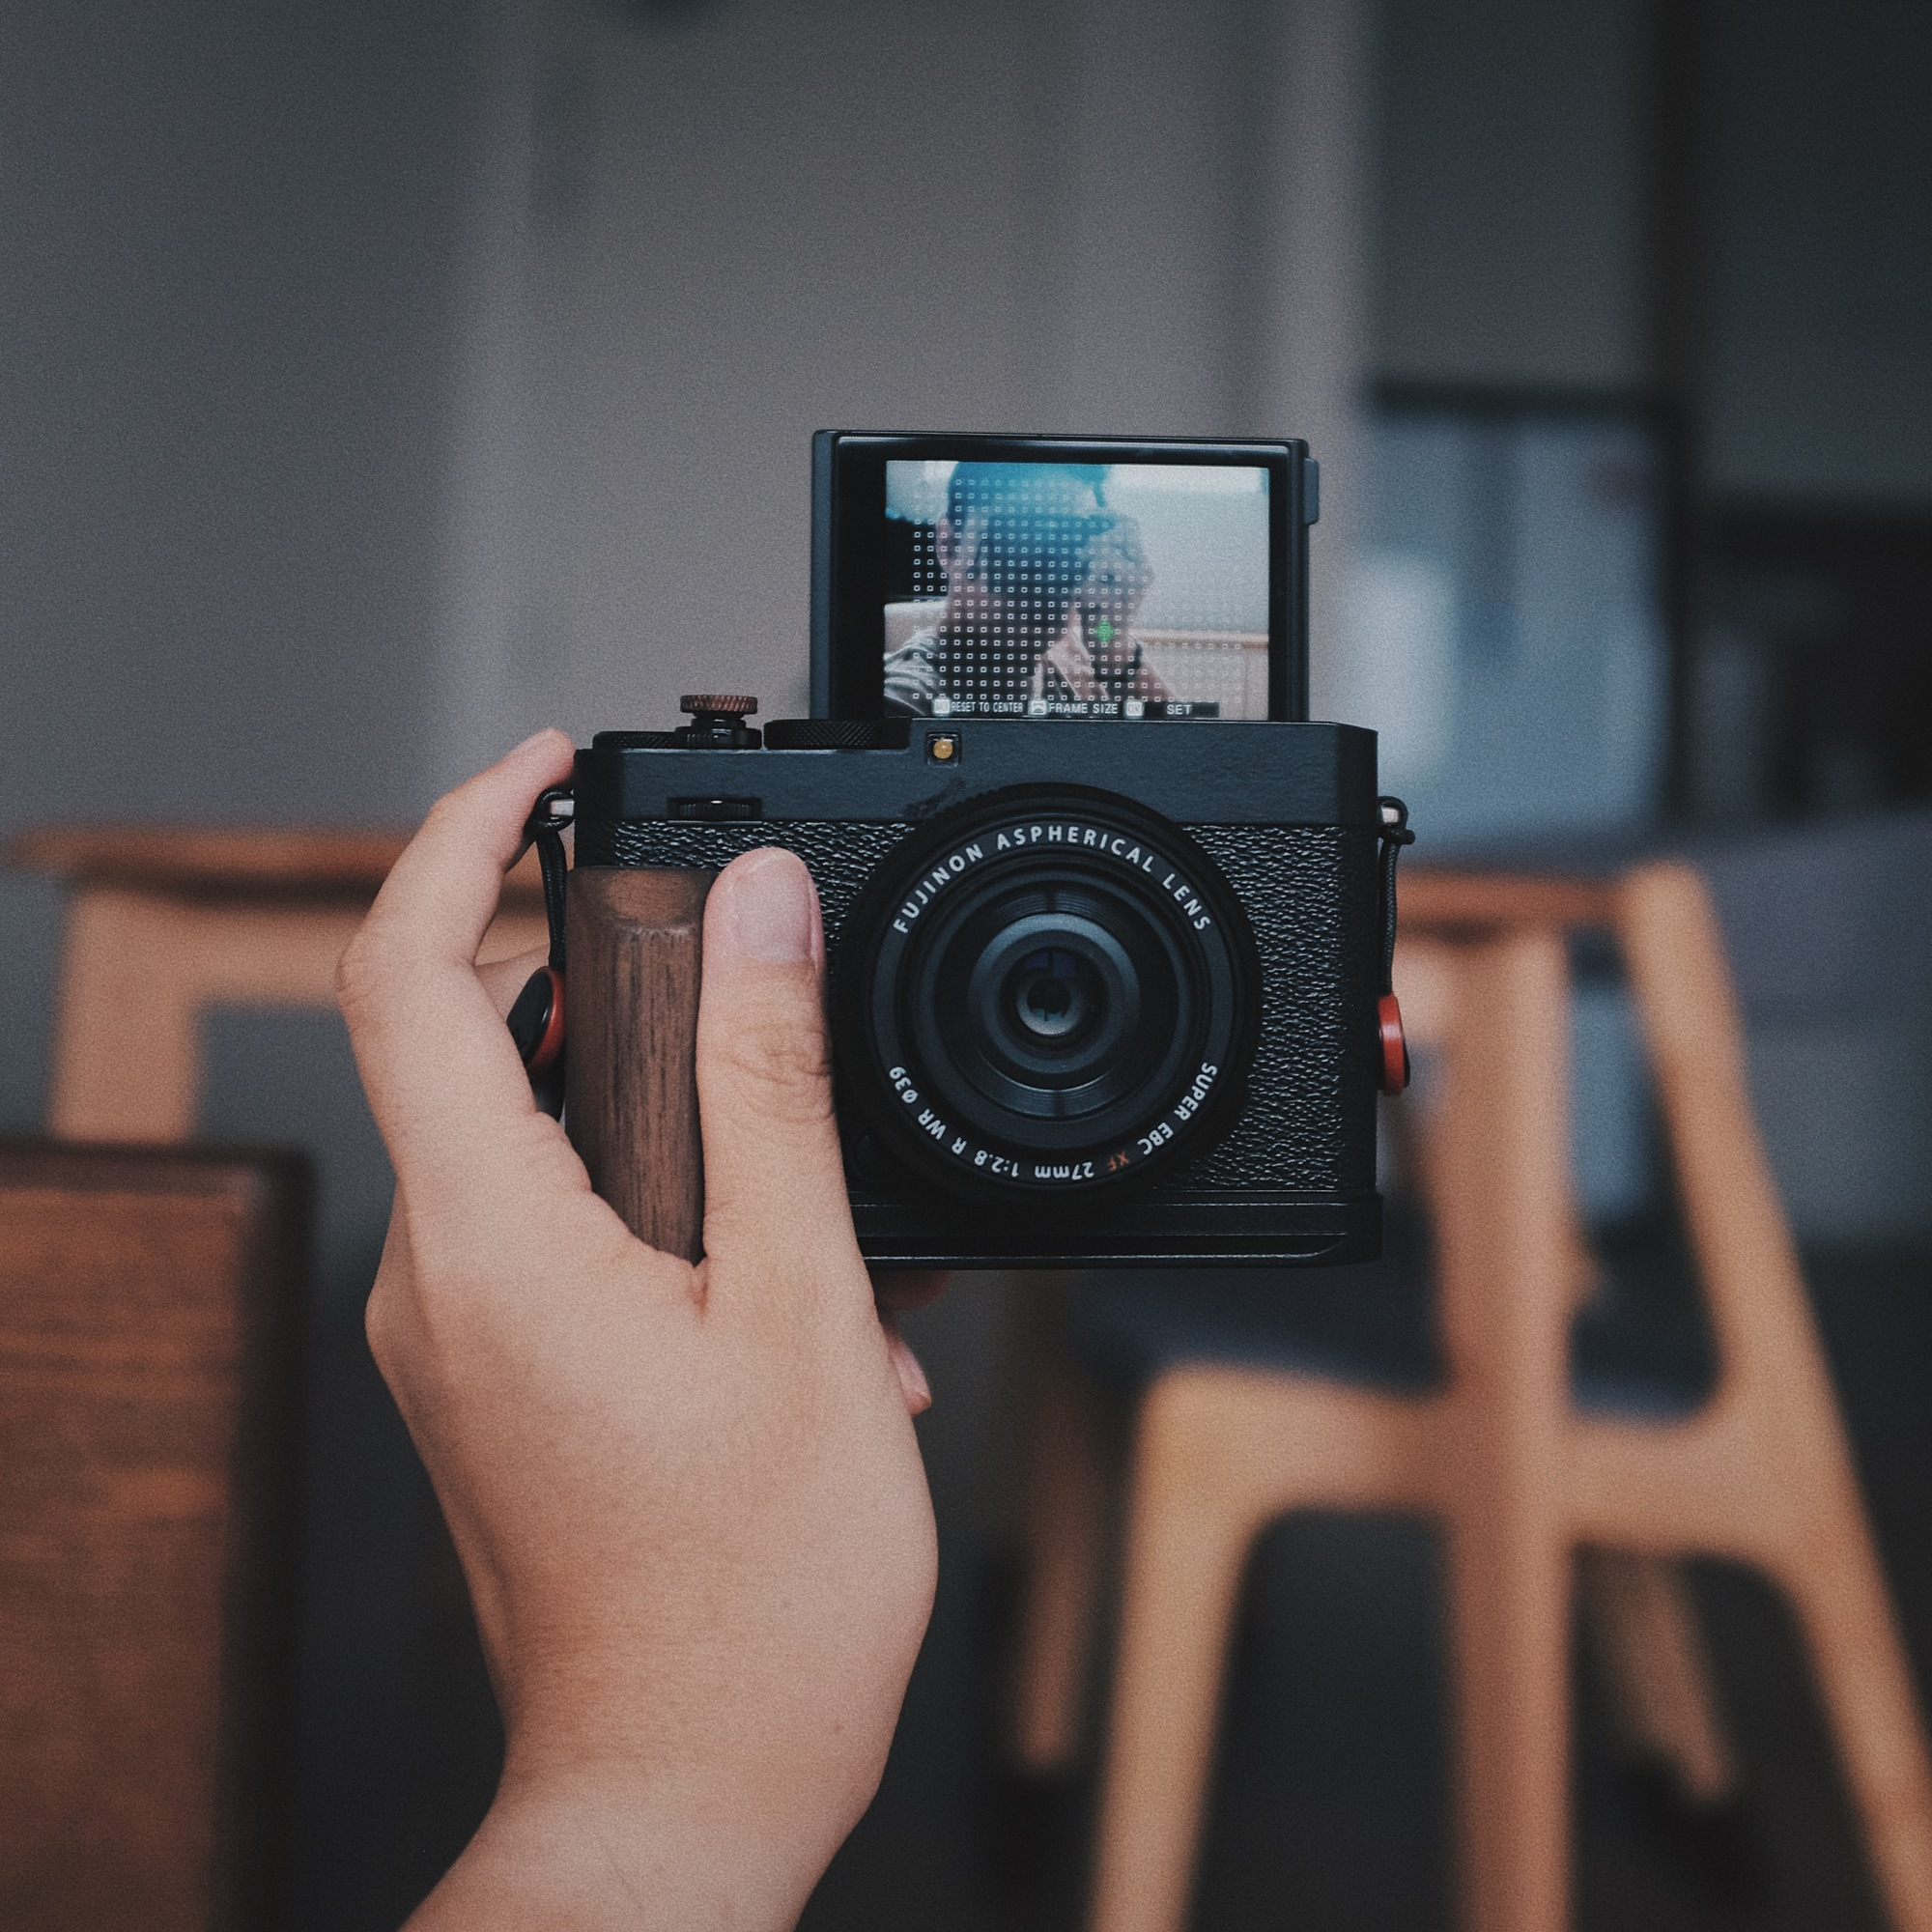
\includegraphics[width=\linewidth]{\envfinaldir/coverpic-prod.jpg}\par
            % \vskip 30pt
            \vfill

            \normalsize\rmfamily\scshape
            \copyright{} The Web Digest Project \hfill\large \envdatestr
        \end{center}
    \end{titlepage}
    % \restoregeometry
}
\newcommand{\simplehref}[1]{%
    \textcolor{blue!80!green}{\href{#1}{#1}}%
}
\renewcommand{\contentsname}{\center\Huge\sffamily\bfseries Contents\par\vskip 20pt}
\newcounter{ipartcounter}
\setcounter{ipartcounter}{0}
\newcommand{\ipart}[1]{
    % \vskip 20pt
    \clearpage
    \stepcounter{ipartcounter}
    \phantomsection
    \addcontentsline{toc}{chapter}{#1}
    % \begin{center}
    %     \Huge
    %     \sffamily\bfseries
    %     #1
    % \end{center}
    % \vskip 20pt plus 7pt
}
\newcounter{ichaptercounter}
\setcounter{ichaptercounter}{0}
\newcommand{\ichapter}[1]{
    % \vskip 20pt
    \clearpage
    \stepcounter{ichaptercounter}
    \phantomsection
    \addcontentsline{toc}{section}{\numberline{\arabic{ichaptercounter}}#1}
    \begin{center}
        \Huge
        \sffamily\bfseries
        #1
    \end{center}
    \vskip 20pt plus 7pt
}
\newcommand{\entrytitlefont}[1]{\subsection*{\raggedright\Large\sffamily\bfseries#1}}
\newcommand{\entryitemGeneric}[2]{
    % argv: title, url
    \parbox{\linewidth}{
        \entrytitlefont{#1}\par\vskip 5pt
        \footnotesize\ttfamily\mdseries
        \simplehref{#2}
    }\vskip 11pt plus 11pt minus 1pt
}
\newcommand{\entryitemGithub}[3]{
    % argv: title, url, desc
    \parbox{\linewidth}{
        \entrytitlefont{#1}\par\vskip 5pt
        \footnotesize\ttfamily\mdseries
        \simplehref{#2}\par\vskip 5pt
        \small\rmfamily\mdseries#3
    }\vskip 11pt plus 11pt minus 1pt
}
\newcommand{\entryitemAp}[3]{
    % argv: title, url, desc
    \parbox{\linewidth}{
        \entrytitlefont{#1}\par\vskip 5pt
        \footnotesize\ttfamily\mdseries
        \simplehref{#2}\par\vskip 5pt
        \small\rmfamily\mdseries#3
    }\vskip 11pt plus 11pt minus 1pt
}
\newcommand{\entryitemHackernews}[3]{
    % argv: title, hnurl, rawurl
    % \parbox{\linewidth}{
    %     \entrytitlefont{#1}\par\vskip 5pt
    %     \footnotesize\ttfamily\mdseries
    %     \simplehref{#3}\par
    %     \textcolor{black!50}{\href{#2}{#2}}
    % }\vskip 11pt plus 11pt minus 1pt
    \begin{minipage}{\linewidth}
            \entrytitlefont{#1}\par\vskip 5pt
            \footnotesize\ttfamily\mdseries
            \simplehref{#3}\par
            \textcolor{black!50}{\href{#2}{#2}}
    \end{minipage}\par\vskip 11pt plus 11pt minus 1pt
}







\begin{document}

\makeheader

\tableofcontents\clearpage




\ipart{Developers}
\ichapter{Hacker News}
\entryitemTwoLinks{Immunotherapy drug clinical trial results: half of tumors shrink or disappear}{https://news.ycombinator.com/item?id=45188945}{https://www.rockefeller.edu/news/38120-immunotherapy-drug-eliminates-aggressive-cancers-in-clinical-trial/}

\entryitemTwoLinks{I still love PHP and JavaScript (2022)}{https://news.ycombinator.com/item?id=45188114}{https://the.scapegoat.dev/why-i-love-php-and-javascript/}

\entryitemTwoLinks{Inflation Erased U.S. Income Gains Last Year}{https://news.ycombinator.com/item?id=45187687}{https://www.wsj.com/economy/consumers/census-income-insurance-poverty-2024-31d82ad0}

\entryitemTwoLinks{A cryptography expert on how Web3 started, and how it's going}{https://news.ycombinator.com/item?id=45186726}{https://spectrum.ieee.org/web3-hardware-security}

\entryitemTwoLinks{Memory Integrity Enforcement}{https://news.ycombinator.com/item?id=45186265}{https://security.apple.com/blog/memory-integrity-enforcement/}

\entryitemTwoLinks{iPhone Air}{https://news.ycombinator.com/item?id=45186015}{https://www.apple.com/newsroom/2025/09/introducing-iphone-air-a-powerful-new-iphone-with-a-breakthrough-design/}

\entryitemTwoLinks{Dropbox Paper mobile App Discontinuation}{https://news.ycombinator.com/item?id=45186011}{https://help.dropbox.com/installs/paper-mobile-discontinuation}

\entryitemTwoLinks{E-paper display reaches the realm of LCD screens}{https://news.ycombinator.com/item?id=45185756}{https://spectrum.ieee.org/e-paper-display-modos}

\entryitemTwoLinks{Microsoft is officially sending employees back to the office}{https://news.ycombinator.com/item?id=45184432}{https://www.businessinsider.com/microsoft-send-employees-back-to-office-rto-remote-work-2025-9}

\entryitemTwoLinks{ICE is using fake cell towers to spy on people's phones}{https://news.ycombinator.com/item?id=45184368}{https://www.forbes.com/sites/the-wiretap/2025/09/09/how-ice-is-using-fake-cell-towers-to-spy-on-peoples-phones/}

\entryitemTwoLinks{U.S. Added 911,000 Fewer Jobs in the Year Ended in March}{https://news.ycombinator.com/item?id=45184315}{https://www.wsj.com/economy/jobs/us-job-growth-revision-a9777d98}

\entryitemTwoLinks{An attacker's blunder gave us a look into their operations}{https://news.ycombinator.com/item?id=45183589}{https://www.huntress.com/blog/rare-look-inside-attacker-operation}

\entryitemTwoLinks{Building a DOOM-like multiplayer shooter in pure SQL}{https://news.ycombinator.com/item?id=45183050}{https://cedardb.com/blog/doomql/}

\entryitemTwoLinks{Source code for the X recommendation algorithm}{https://news.ycombinator.com/item?id=45183039}{https://github.com/twitter/the-algorithm}

\entryitemTwoLinks{We all dodged a bullet}{https://news.ycombinator.com/item?id=45183029}{https://xeiaso.net/notes/2025/we-dodged-a-bullet/}

\entryitemTwoLinks{A new experimental Go API for JSON}{https://news.ycombinator.com/item?id=45182770}{https://go.dev/blog/jsonv2-exp}

\entryitemTwoLinks{US HS students lose ground in math and reading, continuing yearslong decline}{https://news.ycombinator.com/item?id=45182657}{https://apnews.com/article/naep-reading-math-scores-12th-grade-c18d6e3fbc125f12948cc70cb85a520a}

\entryitemTwoLinks{Claude now has access to a server-side container environment}{https://news.ycombinator.com/item?id=45182381}{https://www.anthropic.com/news/create-files}

\entryitemTwoLinks{New Mexico is first state in US to offer universal child care}{https://news.ycombinator.com/item?id=45182372}{https://www.governor.state.nm.us/2025/09/08/new-mexico-is-first-state-in-nation-to-offer-universal-child-care/}

\entryitemTwoLinks{U.S. added 911k fewer jobs in year through March than reported earlier}{https://news.ycombinator.com/item?id=45182111}{https://www.barrons.com/articles/jobs-report-revisions-bls-fed-3d88c77b?st=u8mw75}\ichapter{Phoronix}
\entryitemGeneric{\hskip 0pt{}Rust Coreutils 0.2.2 Released With Faster base64: Outperforming GNU's base64}{https://www.phoronix.com/news/Rust-Coreutils-0.2.2}

\entryitemGeneric{\hskip 0pt{}FEX 2509 Delivers More Performance For x86 Binaries On ARM64 Linux}{https://www.phoronix.com/news/FEX-2509-Released}

\entryitemGeneric{\hskip 0pt{}AMD openSIL Production Phase Reaffirmed For 2026}{https://www.phoronix.com/news/AMD-openSIL-2026}

\entryitemGeneric{\hskip 0pt{}Qualcomm Snapdragon X Elite Linux Performance Improving But Short Of AMD Ryzen \& Intel Core Ultra}{https://www.phoronix.com/review/snapdragon-x1e-september}

\entryitemGeneric{\hskip 0pt{}Ubuntu's Launchpad Deprecating Code Imports From CVS \& Subversion}{https://www.phoronix.com/news/Launchpad-Deprecates-SVN-CVS}

\entryitemGeneric{\hskip 0pt{}NVIDIA CUDA Toolkit 13.0 Update 1 Brings Some Performance Enhancements}{https://www.phoronix.com/news/NVIDIA-CUDA-13.0-Update-1}

\entryitemGeneric{\hskip 0pt{}Linux Sensor Driver Coming For GPD Handhelds}{https://www.phoronix.com/news/GPD-Sensor-Driver-Linux-6.18}

\entryitemGeneric{\hskip 0pt{}Fedora's Modern OS Installer UI Working Well \& Expanding Scope Before Deprecating GTK UI}{https://www.phoronix.com/news/Fedora-Anaconda-WebUI-2025-2026}

\entryitemGeneric{\hskip 0pt{}Fedora 44 Considering Additional Kernel Hardening For Better Security}{https://www.phoronix.com/news/Fedora-44-More-Kernel-Hardening}


\ipart{Developers~~~~(zh-Hans)}
\ichapter{Solidot}
\entryitemGeneric{\hskip 0pt{}Google 同意在韩国对敏感卫星地图进行模糊处理}{https://www.solidot.org/story?sid=82267}

\entryitemGeneric{\hskip 0pt{}空气污染增加路易体痴呆症风险}{https://www.solidot.org/story?sid=82266}

\entryitemGeneric{\hskip 0pt{}移植猪肾的美国男子存活超半年}{https://www.solidot.org/story?sid=82265}

\entryitemGeneric{\hskip 0pt{}农药毒死蜱与儿童大脑异常相关}{https://www.solidot.org/story?sid=82264}

\entryitemGeneric{\hskip 0pt{}尼泊尔取消社媒禁令}{https://www.solidot.org/story?sid=82263}

\entryitemGeneric{\hskip 0pt{}群联称 Windows 11 SSD 问题与早期版本的固件有关}{https://www.solidot.org/story?sid=82262}

\entryitemGeneric{\hskip 0pt{}新汽车电池充电 12 分钟可续航 800 公里}{https://www.solidot.org/story?sid=82261}

\entryitemGeneric{\hskip 0pt{}如何定义超加工食品}{https://www.solidot.org/story?sid=82260}

\entryitemGeneric{\hskip 0pt{}Team Cherry 表示正在改进《空洞骑士:丝之歌》的中文翻译}{https://www.solidot.org/story?sid=82259}

\entryitemGeneric{\hskip 0pt{}周下载量逾 20 亿次的 NPM 包被植入恶意代码}{https://www.solidot.org/story?sid=82258}

\entryitemGeneric{\hskip 0pt{}欧洲最大的论文工厂在乌克兰}{https://www.solidot.org/story?sid=82257}

\entryitemGeneric{\hskip 0pt{}Groklaw 变成了推销加密货币的网站}{https://www.solidot.org/story?sid=82256}

\entryitemGeneric{\hskip 0pt{}酒精如何帮助肠道细菌攻击肝脏}{https://www.solidot.org/story?sid=82255}

\entryitemGeneric{\hskip 0pt{}Red Hat 将后台业务团队迁移到母公司 IBM}{https://www.solidot.org/story?sid=82254}

\entryitemGeneric{\hskip 0pt{}尼泊尔年轻人抗议社交媒体禁令}{https://www.solidot.org/story?sid=82253}

\entryitemGeneric{\hskip 0pt{}82\% 的澳大利亚人玩游戏}{https://www.solidot.org/story?sid=82252}

\entryitemGeneric{\hskip 0pt{}天文学家在矮星系发现偏离中心的黑洞}{https://www.solidot.org/story?sid=82251}

\entryitemGeneric{\hskip 0pt{}红海海底光缆事故扰乱微软 Azure 云服务 }{https://www.solidot.org/story?sid=82250}

\entryitemGeneric{\hskip 0pt{}亚马逊制作《奇异人生》真人版}{https://www.solidot.org/story?sid=82249}

\entryitemGeneric{\hskip 0pt{}土耳其限制大部分社交媒体}{https://www.solidot.org/story?sid=82248}\ichapter{V2EX}
\entryitemGeneric{\hskip 0pt{}[Apple] 对 iPhone Air 动心了,发愁 esim 到底怎么个情况}{https://www.v2ex.com/t/1158150}

\entryitemGeneric{\hskip 0pt{}[Google] google 账号登录不了 重金酬谢}{https://www.v2ex.com/t/1158148}

\entryitemGeneric{\hskip 0pt{}[iPhone] 17air 的 esim 能接受非联通的短信转发吗?}{https://www.v2ex.com/t/1158147}

\entryitemGeneric{\hskip 0pt{}[Apple] 纯 esim 真的比 sim 卡好吗?}{https://www.v2ex.com/t/1158145}

\entryitemGeneric{\hskip 0pt{}[Apple] 哪个地区版本的 iPhone 17/17 Pro 功能最全}{https://www.v2ex.com/t/1158144}

\entryitemGeneric{\hskip 0pt{}[Apple] 没想到港版 iPhone 17 Pro 才是最适合我的版本}{https://www.v2ex.com/t/1158143}

\entryitemGeneric{\hskip 0pt{}[Apple] 关于 esim 政策,想买 iPhone Air 的进来看看怎么选择?}{https://www.v2ex.com/t/1158142}

\entryitemGeneric{\hskip 0pt{}[iPhone] iPhone 14Pro 换 17 是不是全方位提升}{https://www.v2ex.com/t/1158141}

\entryitemGeneric{\hskip 0pt{}[分享创造] 和小伙伴自研加密货币交易所系统(Golang + Vue3 Ionic), 23 年至今}{https://www.v2ex.com/t/1158140}

\entryitemGeneric{\hskip 0pt{}[Apple] 今年日版 iPhone 全系列不支持物理 SIM,仅支持 eSIM}{https://www.v2ex.com/t/1158139}

\entryitemGeneric{\hskip 0pt{}[ WATCH] 又一年过去了, Apple Watch 还是不支持快充}{https://www.v2ex.com/t/1158138}

\entryitemGeneric{\hskip 0pt{}[Apple] iPhone 各型号价格一图流,标准版 5999 起, Pro Max 最高 2TB 存储}{https://www.v2ex.com/t/1158137}

\entryitemGeneric{\hskip 0pt{}[Apple] 17 的标准版和 air 比较值得买}{https://www.v2ex.com/t/1158136}

\entryitemGeneric{\hskip 0pt{}[Apple] iPhone 17 系列国行价格,全系 256GB 起}{https://www.v2ex.com/t/1158135}

\entryitemGeneric{\hskip 0pt{}[iPhone] 如果 Apple 智能将来在中国推出,我在中国购买的 iPhone 系列机型能启用 Apple 智能吗?}{https://www.v2ex.com/t/1158134}

\entryitemGeneric{\hskip 0pt{}[Apple] iPhone 17 标准版 可以算牙膏挤爆了}{https://www.v2ex.com/t/1158133}

\entryitemGeneric{\hskip 0pt{}[Apple] 17Air 的 esim「在中国大陆仅支持激活型号 A3518」}{https://www.v2ex.com/t/1158132}

\entryitemGeneric{\hskip 0pt{}[Apple] 妈蛋,我今年刚换的 16pro 啊,问下能不能去国外 trade in}{https://www.v2ex.com/t/1158131}

\entryitemGeneric{\hskip 0pt{}[问与答] 橙色 iPhone 17 Pro 是真心好看}{https://www.v2ex.com/t/1158130}

\entryitemGeneric{\hskip 0pt{}[Apple] iPhone 17 标准版终于上 120hz 高刷了}{https://www.v2ex.com/t/1158129}

\entryitemGeneric{\hskip 0pt{}[Apple] Airpods Pro3 发布了,降噪提升至 2 倍,续航提升至 8 小时,感觉很值得换?}{https://www.v2ex.com/t/1158128}

\entryitemGeneric{\hskip 0pt{}[微软] Visual Studio 2026 来了~~~~~~}{https://www.v2ex.com/t/1158127}

\entryitemGeneric{\hskip 0pt{}[问与答] 兄弟们,我被网路黑客盯上了。hotmail 邮箱一直收到大量不明的网站订阅信息}{https://www.v2ex.com/t/1158125}

\entryitemGeneric{\hskip 0pt{}[职场话题] 如何带社招新人?}{https://www.v2ex.com/t/1158123}

\entryitemGeneric{\hskip 0pt{}[问与答] 串流可以买采集卡来提升刷新率吗}{https://www.v2ex.com/t/1158121}

\entryitemGeneric{\hskip 0pt{}[汽车] 有人了解 2025 本田皓影 phev 这款 suv 么?值得拥有吗?}{https://www.v2ex.com/t/1158120}

\entryitemGeneric{\hskip 0pt{}[推广] 整理了 12 个 Nano Banana 免费平台(部分有次数限制)}{https://www.v2ex.com/t/1158119}

\entryitemGeneric{\hskip 0pt{}[酷工作] [深圳前海] 招聘熟悉 Next.js 前端}{https://www.v2ex.com/t/1158118}

\entryitemGeneric{\hskip 0pt{}[宽带症候群] anytls+reality 有人被 ban 过吗?}{https://www.v2ex.com/t/1158117}

\entryitemGeneric{\hskip 0pt{}[宽带症候群] immortalwrt 系统遇到的问题,求助}{https://www.v2ex.com/t/1158115}

\entryitemGeneric{\hskip 0pt{}[Solana] 请问下大佬怎么定投加密货币}{https://www.v2ex.com/t/1158114}

\entryitemGeneric{\hskip 0pt{}[程序员] 批量下载 sourceforge 的小工具}{https://www.v2ex.com/t/1158113}

\entryitemGeneric{\hskip 0pt{}[酷工作] [社招] 大厂 AGI 团队 高薪 预训练、后训练、agent 算法专家}{https://www.v2ex.com/t/1158111}

\entryitemGeneric{\hskip 0pt{}[分享创造] 将任意书籍转换为 rime 词库}{https://www.v2ex.com/t/1158110}

\entryitemGeneric{\hskip 0pt{}[VXNA] 申请博客收录}{https://www.v2ex.com/t/1158109}

\entryitemGeneric{\hskip 0pt{}[宽带症候群] 有人用过海外这种 IPTV 吗? 4w 个频道,价格也不高,不过好像在国内直连一般般}{https://www.v2ex.com/t/1158108}

\entryitemGeneric{\hskip 0pt{}[macOS] 有啥 App 能做到长按 cmd 键呼出 App Switcher,并能通过数字键打开对应的 App 吗?}{https://www.v2ex.com/t/1158107}

\entryitemGeneric{\hskip 0pt{}[Solana] 基于 CUDA 的计算 Solana 虚荣地址的程序}{https://www.v2ex.com/t/1158105}

\entryitemGeneric{\hskip 0pt{}[推广] 给找工作困难的人写的一份指南(看出狱后找不到工作的随笔)}{https://www.v2ex.com/t/1158104}

\entryitemGeneric{\hskip 0pt{}[电影] 有人看过余命十年吗?看电影从来没哭过的看哭了😭}{https://www.v2ex.com/t/1158103}

\entryitemGeneric{\hskip 0pt{}[问与答] 现在 google nano banana 比较火爆 想在国内调用}{https://www.v2ex.com/t/1158102}

\entryitemGeneric{\hskip 0pt{}[Local LLM] 大模型上下文工程实践指南-第 3 章:提示词技术}{https://www.v2ex.com/t/1158100}

\entryitemGeneric{\hskip 0pt{}[Android] [原创] 分享一个 Android SO 分析小工具}{https://www.v2ex.com/t/1158099}

\entryitemGeneric{\hskip 0pt{}[分享创造] 我做了个 网站出海 SEO 关键词挖掘工具,简单好用,能发觉新需求!}{https://www.v2ex.com/t/1158097}

\entryitemGeneric{\hskip 0pt{}[酷工作] 寻找一位有经验的产品经理加入我们团队}{https://www.v2ex.com/t/1158096}

\entryitemGeneric{\hskip 0pt{}[上海] 上海塘镇地铁站附件上班,哪里租房性价比高呢}{https://www.v2ex.com/t/1158095}

\entryitemGeneric{\hskip 0pt{}[问与答] 有哪些好用的 nano-banana api , 不需要科学上网的。求推荐啊。我要买。}{https://www.v2ex.com/t/1158094}

\entryitemGeneric{\hskip 0pt{}[健康] 肺 CA 晚期,有没有老哥有买药途径的?}{https://www.v2ex.com/t/1158093}

\entryitemGeneric{\hskip 0pt{}[成都] 成都远程工作者进来交流一下}{https://www.v2ex.com/t/1158092}

\entryitemGeneric{\hskip 0pt{}[美酒与美食] V2 的石榴老哥,今年还卖石榴吗}{https://www.v2ex.com/t/1158091}


\ipart{Generic News}







\clearpage
\leavevmode\vfill
\footnotesize

Copyright \copyright{} 2023-2025 Neruthes and other contributors.

This document is published with CC BY-NC-ND 4.0 license.

The entries listed in this newsletter may be copyrighted by their respective creators.

This newsletter is generated by the Web Digest project.

The newsletters are also delivered via Telegram channel \CJKunderline{\href{https://t.me/webdigestchannel}{https://t.me/webdigestchannel}}.\\
RSS feed is available at \CJKunderline{\href{https://webdigest.pages.dev/rss.xml}{https://webdigest.pages.dev/rss.xml}}.

This newsletter is available in PDF at
\CJKunderline{\href{https://webdigest.pages.dev/}{https://webdigest.pages.dev/}}.

The source code being used to generate this newsletter is available at\\
\CJKunderline{\href{https://github.com/neruthes/webdigest}{https://github.com/neruthes/webdigest}}.

This newsletter is also available in
\CJKunderline{\href{http://webdigest.pages.dev/readhtml/\envyear/WebDigest-20250910.html}{HTML}} and
\CJKunderline{\href{https://github.com/neruthes/webdigest/blob/master/markdown/\envyear/WebDigest-20250910.md}{Markdown}}.


\coverpic{https://unsplash.com/photos/a-bird-perched-on-top-of-a-pine-tree-INrsmwGcfyw}{Emma Swoboda}


\end{document}
